
The goal here is to compute the time evolution of the concurrence \( C(\rho(t)) \) in the lattice 
as shown in \refig{fig:Schematic of the lattice of the spin chain}, 
with the Hamiltonian of the XY model and DMI.
To achieve this, we have two approaches: a numerical approach using the Python programming language and an analytical approach.


\subsection{Numerical approch}
To simulate the evolution of the concurrence \refdef{def: concurrence}, we need to compute the 
density matrix. However, the necessary 
condition to compute the density matrix \( \rho(t) \) is to find 
the state of the quantum system at time \( t \). For this purpose, 
we use the postulate of the evolution of the quantum system given by the Schrödinger equation \cite{cohen-tannoudji_quantum_2019}. 



\begin{equation}\label{eq: Schrodinger eq}
    \forall t \in \mathbb{R}_+, \ i \hbar \partial_t \ket{\psi(t)} = \hamil(t) \ket{\psi (t)} 
\end{equation}

Now let's explain a generic algorithm to solve the Schrödinger equation.

First, let's introduce the evolution operator \( \mathcal{U}(t, t_0) \) which maps the initial state 
\( \ket{\psi(t_0)} \) of 
the system to the state \( \ket{\psi(t)} \) at time \( t \):  

\begin{equation}\label{def : evolution operator}
   \forall t \in \mathbb{R}_+, \ \ketpsit = \opevolution{t_0}  \ket{\psi(t_0)} 
   \text{ with  } \ \opevolution{t_0} \opevolution{t_0}^\dagger = \opevolution{t_0}^\dagger \opevolution{t_0} = \text{id}  
\end{equation}

where \( \text{id} \) is the identity operator and \( \mathcal{U}^\dagger(t, t_0) \) is the adjoint of \( \mathcal{U}(t, t_0) \).
Now, let's consider a Hamiltonian \( \hamil(t) \) which is piecewise constant, i.e.,



\begin{equation}\label{prop: hypothese Hamiltionan}
    \forall j \in \mathbb{N}, \  \hamil(t) = \hamil(t_j) \quad \text{for} \quad t_j < t < t_{j+1},     
\end{equation}

where \( t_j \) are time steps at which the Hamiltonian changes suddenly.
\graphli{0.7}{methodology/constante_H.pdf}{Schematic of the \refprop{prop: hypothese Hamiltionan}}{hypothese Hamiltionan}

With the hypothesis in \refprop{prop: hypothese Hamiltionan}, the evolution operator in \refdef{def : evolution operator}, 
and the Schrödinger equation in \myeqref{eq: Schrodinger eq}, we can express the evolution operator \( \mathcal{U}(t, t_0) \) as:


\begin{equation}
    \opevolution{t_0} = e^{-i \hamil (t-t_0)/\hbar}
\end{equation}



With the hypothesis in \refprop{prop: hypothese Hamiltionan}, the evolution operator in \refdef{def : evolution operator}, and the 
Schrödinger equation in \myeqref{eq: Schrodinger eq}, we can express the evolution operator \( \mathcal{U}(t, t_0) \) as:

\begin{align*}
    \ketpsitime{t_1} &= e^{-i \hamil (t_0) (t_1-t_0)/\hbar} \ketpsitime{t_0} \\
    \ketpsitime{t_2} &= e^{-i \hamil (t_1) (t_2-t_1)/\hbar} \ketpsitime{t_1} =  e^{-i \hamil(t_1) (t_2-t_1)/\hbar} 
    e^{-i \hamil(t_0) (t_1-t_0)/\hbar} \ketpsitime{t_0}\\
    &\vdots \\
    \ketpsitime{t_n} &= e^{-i \hamil(t_{n-1}) (t_n-t_{n-1})/\hbar} \ketpsitime{t_{n-1}} \cdots  e^{-i \hamil(t_{0}) (t_2-t_1)/\hbar} 
    e^{-i \hamil (t_1-t_0)/\hbar} \ketpsitime{t_0}
\end{align*}

Let us consider equally spaced time intervals:

\[
t_j = t_0 + j \Delta t.
\]

Thus, the state of the quantum system at time \( t_n \) is:
\begin{equation} \label{eq: expression state t_n}
   \forall n \in \mathbb{N}^*, \  \ketpsitime{t_n} = \prod_{i=0}^{n-1} e^{-i \hamil(t_{i}) \Delta t /\hbar} \ketpsitime{t_0}
\end{equation}

Notice the temporal order of operators \( \mathcal{U}(t_j, t_{j-1}) \) with \( t_j > t_{j-1} \). Operators later in time appear to the left.

From this, we can deduce the following algorithm to solve the Schrödinger equation:
\begin{algorithm}[H]
    \caption{Solve Time-Dependent Schrödinger Equation}
    \begin{algorithmic}[1]
    \Procedure{solve}{$n: \text{integer}, t_f: \text{integer}, \text{Hamil: function}, \ketpsitime{t_0}: \text{array}$}
    \State $\Delta t \gets \frac{t_f}{n}$
    \State $\text{times} \gets \text{linspace}(0, t_f, n)$
    \State $\text{state\_t} \gets \text{empty list}$
    
    \For{$j = 0$ \textbf{to} $\text{length of times} - 1$}
        \State $\hamil(t_j) \gets \text{Hamil(times}[j])$
        \State $\mathcal{U}(t_{j+1}-t_j) \gets \text{matrix\_exponential}\left(-i \times \hamil(t_j) \times \Delta t \right)$
        \State $\ket{\psi(t_{j+1})} \gets \text{matrix\_dot\_product}(\mathcal{U}(t_{j+1}-t_j), \ket{\psi(t_0)})$
        \State \text{append } $\ket{\psi(t_{j+1})}$ \text{ to state\_t}
        \State $\ket{\psi(t_0)} \gets \ket{\psi(t_{j+1})}$
    \EndFor
    
    \State \Return $\text{state\_t}$
    \EndProcedure
    \end{algorithmic}
\end{algorithm}

\newpage 


Now we can compute the density matrix at time \( t \). However, if the length of the lattice is \( L>1 \), we cannot 
compute \( C(\rho(t)) \) directly according to the definition of concurrence \refdef{def: concurrence}, which applies to only two qubits. If \( L>1 \), 
there are more than two qubits in the lattice, so the standard definition of concurrence cannot be used. 
Let's examine an example with three qubits to understand this problem, as shown in the following figure:


\begin{figure}[h!]
    \centering
    \begin{subfigure}[b]{0.3\textwidth}
        \centering
        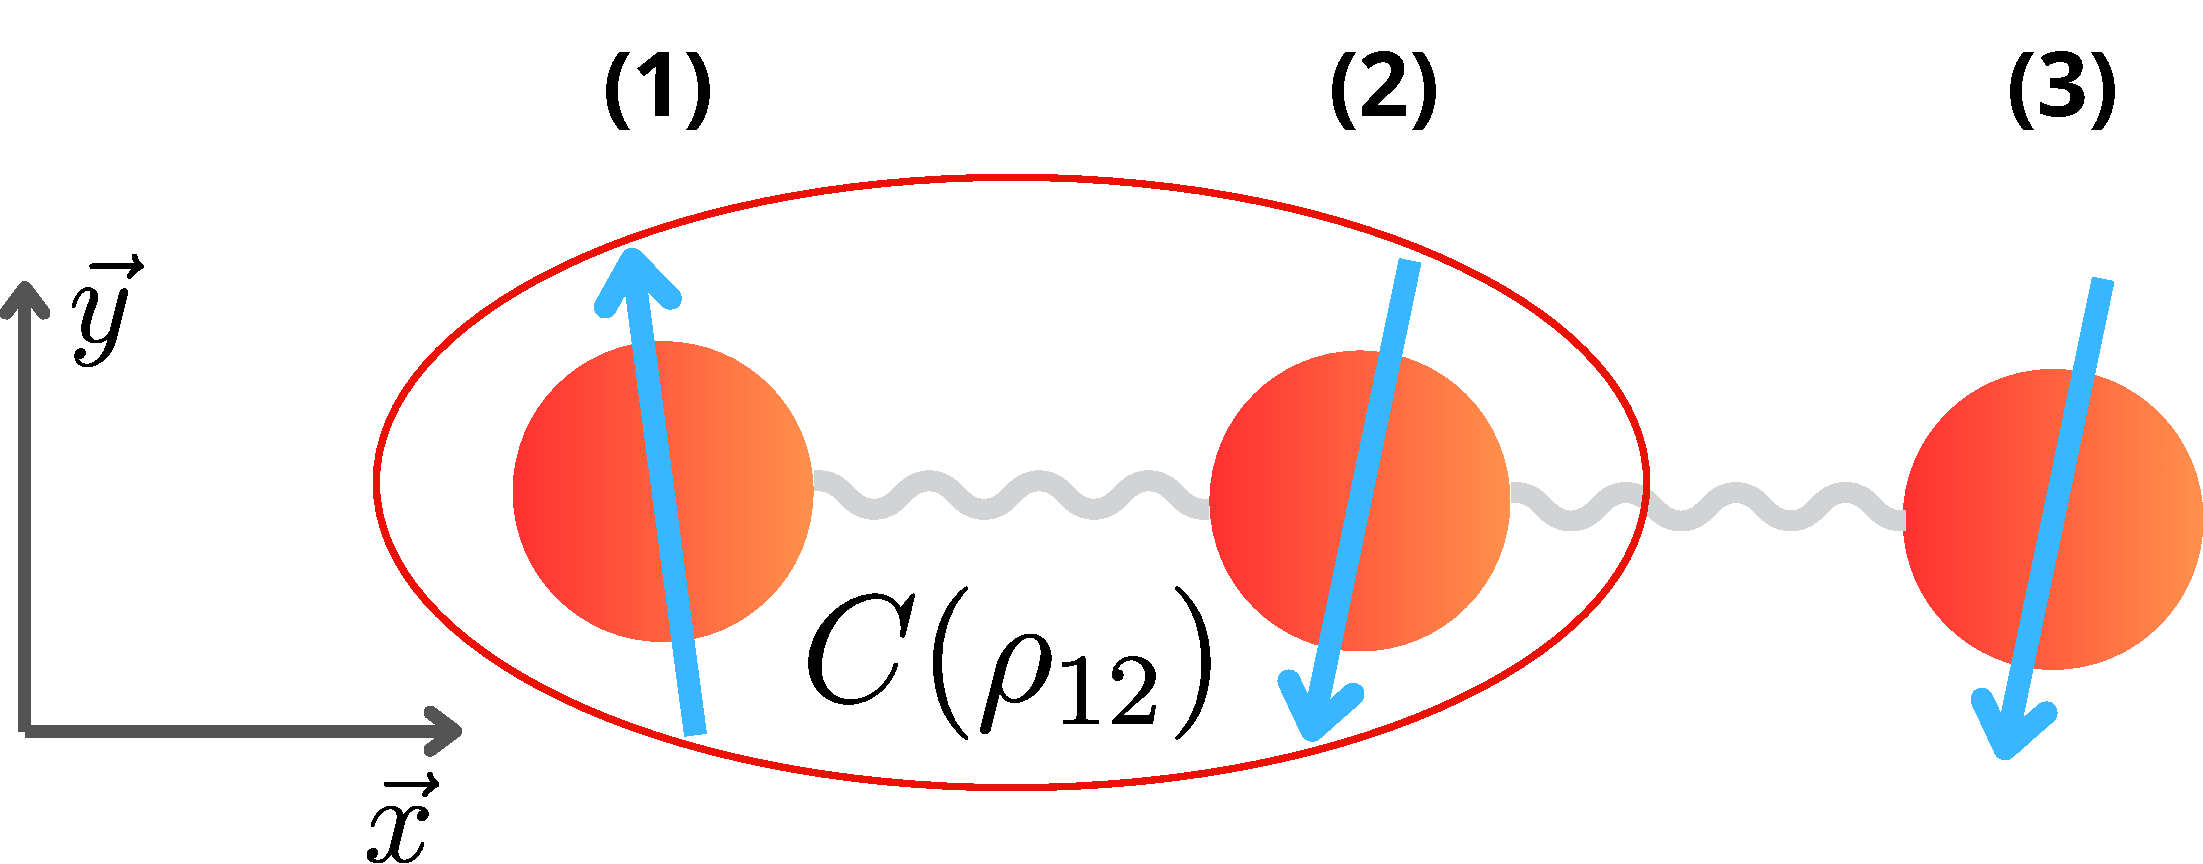
\includegraphics[width=\textwidth]{methodology/partial_trace_1.pdf}
        \caption{\centering Concurrence between the qubit (1) and (2)}
        \label{fig:Concurrence between the qubit (1) and (2)}
    \end{subfigure}
    \hfill
    \begin{subfigure}[b]{0.3\textwidth}
        \centering
        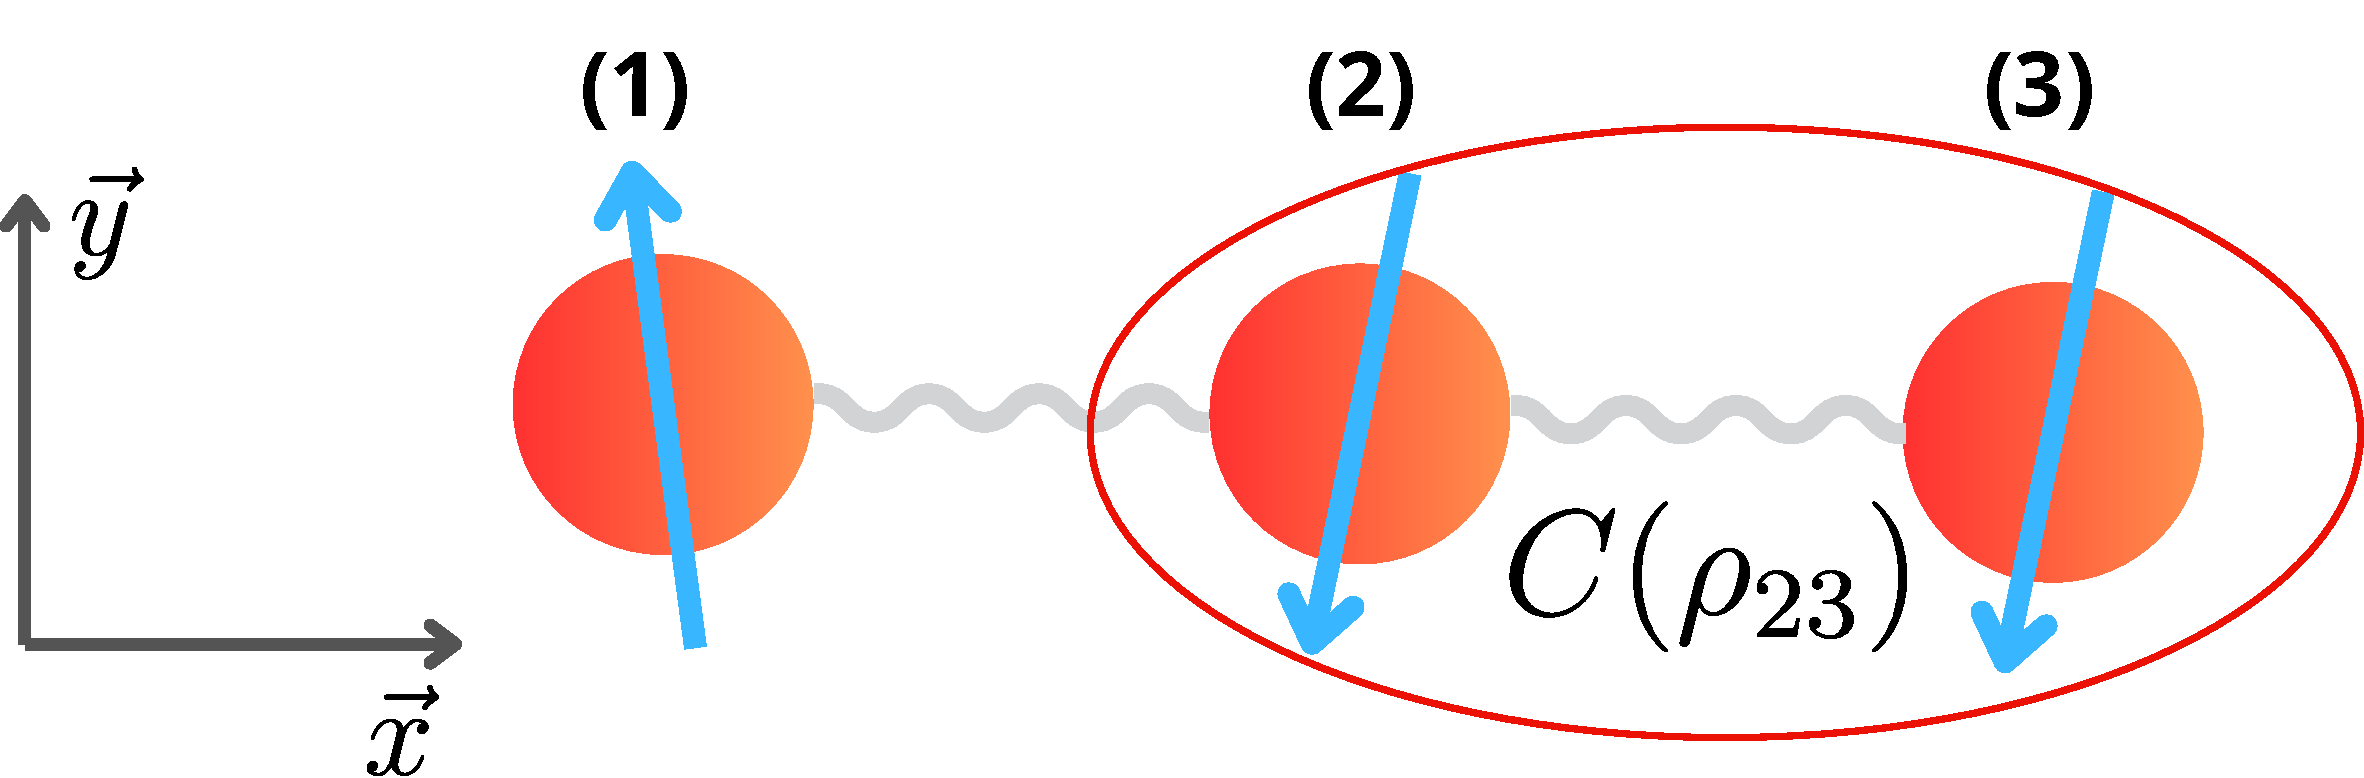
\includegraphics[width=\textwidth]{methodology/partial_trace_2.pdf}
        \caption{\centering Concurrence between the qubit (2) and (3)}
        \label{fig:Concurrence between the qubit (2) and (3)}
    \end{subfigure}
    \hfill
    \begin{subfigure}[b]{0.3\textwidth}
        \centering
        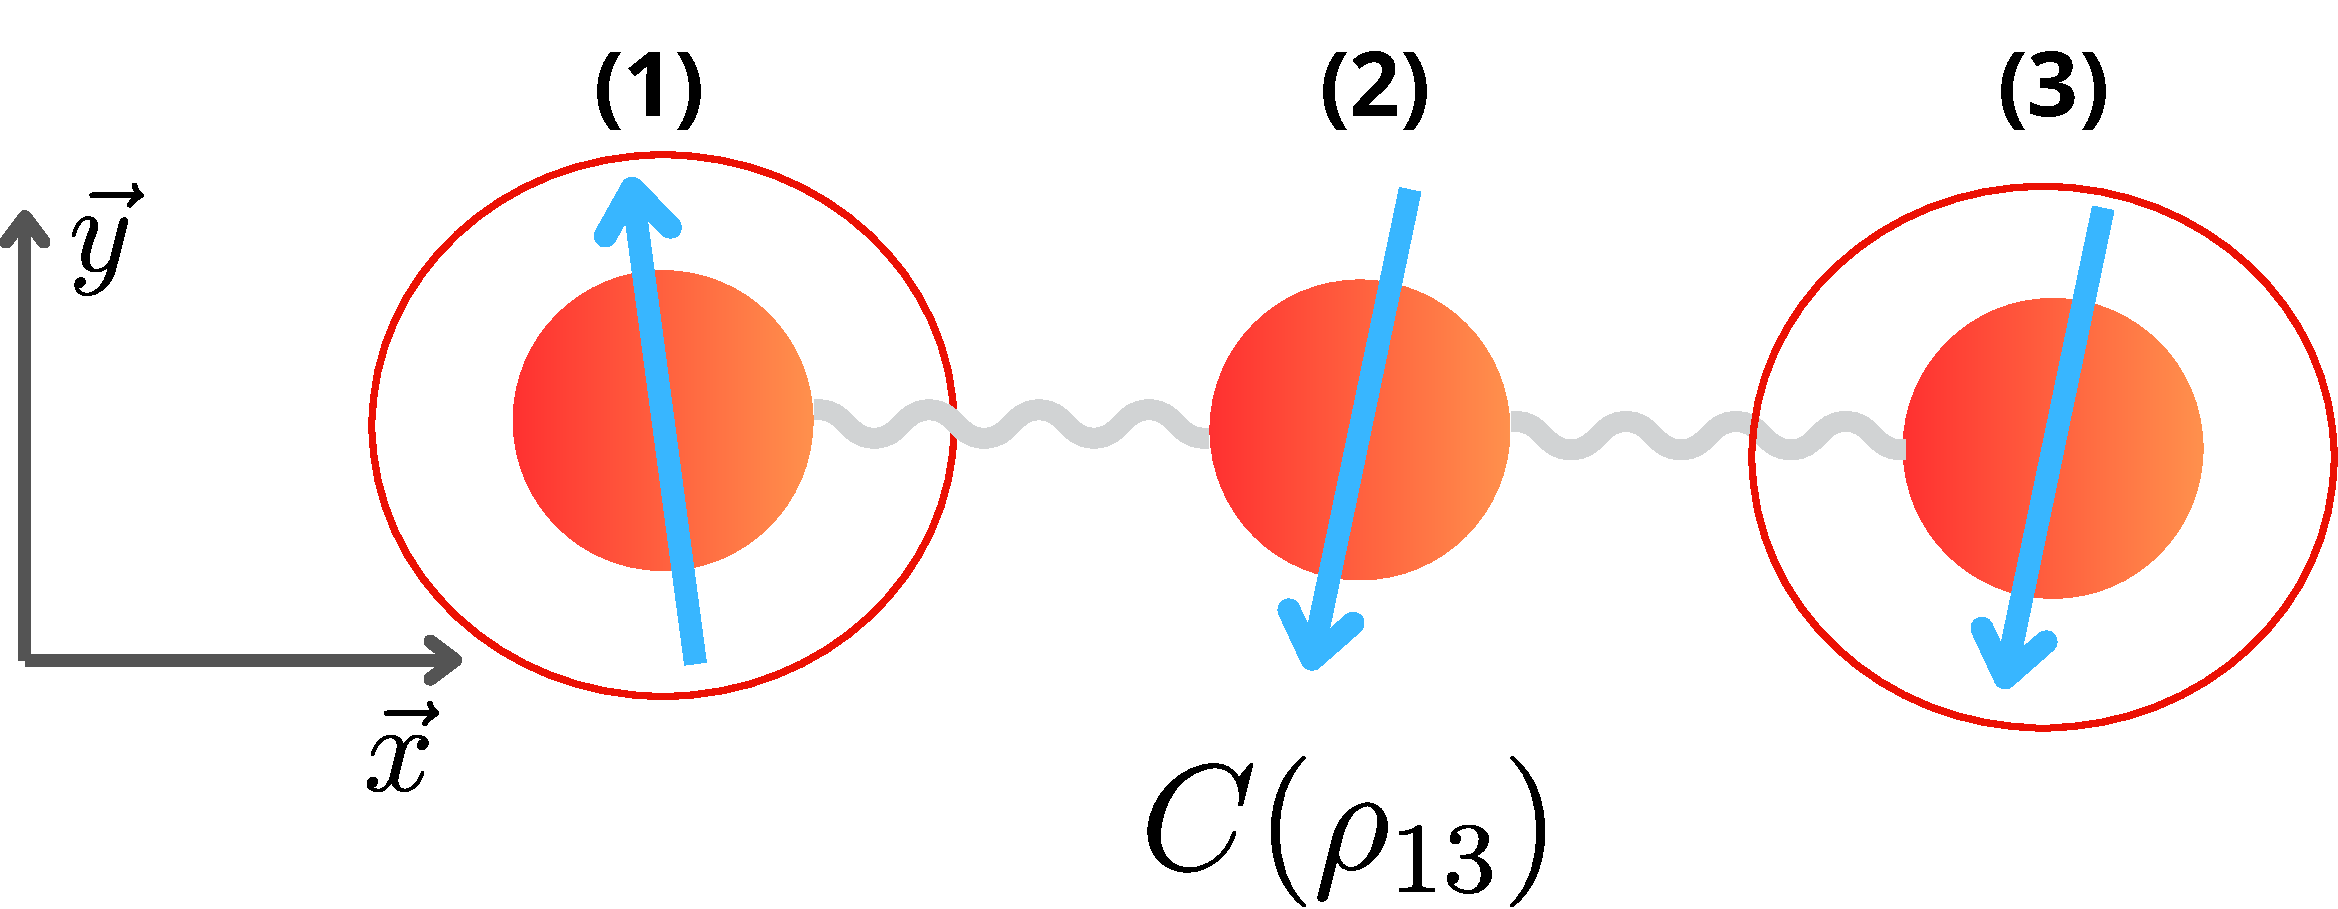
\includegraphics[width=\textwidth]{methodology/partial_trace_3.pdf}
        \caption{\centering Concurrence between the qubit (1) and (3)}
        \label{fig:Concurrence between the qubit (1) and (3)}
    \end{subfigure}
    \caption{Problem of calculation of the concurrence for many qubits}
    \label{fig:partial_traces}
\end{figure}



As seen in \ref{fig:partial_traces}, we need to isolate 
pairs of qubits and compute the density matrix of each pair, denoted as 
\( \rho_{ij} \) where \( i \neq j \text{ and } (i,j) \in \mathbb{N}^* \). 
For this, we use a mathematical tool called the partial trace \cite{bradley_at_2020}.



Let $A$ and $B$ be two subsystems making up the composite system described by the density operator 
$\rho_{AB} \in \mathcal{M}_{2^N}(\mathbb{C})$.
Let note $\dim(\mathcal{H}_A) = d_A$ and $\dim(\mathcal{H}_B) = d_B$.

The partial trace over the $B$ subsystem, denoted $\text{Tr}_B$, is defined as
\begin{equation}\label{eq: partial trace}
\text{Tr}_B[\rho_{AB}] := \sum_j^{d_B} (\id{d_A}{A} \otimes \langle j|_B) \rho_{AB} (\id{d_A}{A} \otimes |j\rangle_B), 
\end{equation}
where $\{|j\rangle\}$ is any orthonormal basis for the Hilbert space $\mathcal{H}_B$ of subsystem $B$. 
We often write $\rho_A \equiv \text{Tr}_B[\rho_{AB}] \in \mathcal{M}_{2^{(N-1)}}(\mathbb{C})$ and $\id{d_A}{A}$ the identity
matrix size $d_A$. 




Similarly, the partial trace over the $A$ subsystem, denoted $\text{Tr}_A$, is defined as
\begin{equation}
\text{Tr}_A[\rho_{AB}] := \sum_j^{d_A} (\langle i|_A \otimes \id{d_B}{B}) \rho_{AB} (|i\rangle_A \otimes \id{d_B}{B}), 
\end{equation}
where $\{|i\rangle\}$ is any orthonormal basis for the Hilbert space $\mathcal{H}_A$ of subsystem $A$. 
We often write $\rho_B \equiv \text{Tr}_A[\rho_{AB}] \in \mathcal{M}_{2^{(N-1)}}(\mathbb{C})$ and $\id{d_A}{A}$ the identity
matrix size $d_B$. 
 .







